% Official CS5228 IEEEtran template, downloaded from Canvas 23 October 2026.
% Outline: motivation -> data/EDA -> methods -> local validation -> interpretation.
% This is the single evolving final-report source. No training is performed here.
\documentclass[conference]{IEEEtran}
\IEEEoverridecommandlockouts
\usepackage{cite}
\usepackage{amsmath,amssymb,amsfonts}
\usepackage{graphicx}
\usepackage{textcomp}
\usepackage{xcolor}
\usepackage{booktabs}
\usepackage{tikz}
\usepackage[hidelinks]{hyperref}
\hypersetup{pdftitle={Predicting Singapore HDB Rents with Comparable Transactions and Temporally Diverse Ensembles},pdfauthor={Han Linxuan; Sun Shenghe; Zhang Yuhong; Zhang Zhexuan}}
\pagestyle{plain}
\newcommand{\code}[1]{\texttt{\small #1}}
\begin{document}

\title{Predicting Singapore HDB Rents with Comparable Transactions and Temporally Diverse Ensembles%
\thanks{CS5228 Group 44, National University of Singapore. Results reflect experiments completed through 6 October 2026.}}
\author{\IEEEauthorblockN{Han Linxuan}\IEEEauthorblockA{A0350911M}
\and\IEEEauthorblockN{Sun Shenghe}\IEEEauthorblockA{A0354849L}
\and\IEEEauthorblockN{Zhang Yuhong}\IEEEauthorblockA{A0356795H}
\and\IEEEauthorblockN{Zhang Zhexuan}\IEEEauthorblockA{A0355290A}}
\maketitle
\thispagestyle{plain}

\begin{abstract}
We investigate monthly rental prediction for Singapore Housing and Development Board flats using 150,000 labelled transactions. The main challenges are market change, heterogeneous flats and the absence of reliable individual-flat identifiers. Consistent preprocessing and spatial joins support comparable-transaction statistics; market adjustment and training-history augmentation then provide complementary inputs to an eight-component CatBoost ensemble. On January--March 2025 it achieves RMSE 440.76 and MAE 316.55 SGD, versus RMSE 445.52 for a four-component market-adjusted reference. Gains also appear in two longer development windows, but an older annual window worsens by 9.81 RMSE. Transactions at or below 2,500 SGD contribute 52.23\% of recent squared error despite representing only 16.34\% of observations. Further model and information screens do not establish a stable replacement. The study therefore documents both useful comparable-market information and the limits of transferring recent gains across market periods.
\end{abstract}
\begin{IEEEkeywords}
HDB rental prediction, tabular regression, comparable transactions, temporal validation, ensemble learning
\end{IEEEkeywords}

\section{Introduction}
Predicting a plausible monthly rent can help renters compare options and help owners assess an asking price. In Singapore's public housing market, a prediction must account for the physical flat and its surroundings, while recognising that the same nominal amount has different market meaning at different dates. A large flat far from transport and a smaller flat near a commercial centre may attract similar rents. We aim to estimate recorded monthly rent from observable transaction characteristics and to explain where those estimates remain unreliable.

The course provides a regression task built from HDB rental approval information and auxiliary datasets\cite{course}. We treat it as dated cross-sectional transaction prediction. The underlying process may contain repeated observations of individual flats, but the released fields do not establish those identities. Several flats in a block can share their type, model and area. A block-level rental history is therefore evidence about comparable transactions, not a verified trajectory for one flat. This distinction matters both when handling repeated records and when interpreting historical features.

Three research questions organise the study. \textit{RQ1:} What information is recovered through consistent preprocessing and spatial joins? \textit{RQ2:} Do market-adjusted comparable rents and different training-history views improve local prediction? \textit{RQ3:} Do these improvements transfer across periods, and which groups account for the remaining errors? Local chronological evaluation and interpretation are our primary evidence; competition scores provide a supplementary external check.

Our contribution is an empirical workflow rather than a new boosting algorithm. We document (1) an auditable treatment of categories, spatial joins and ambiguous repeats; (2) a reproducible predictor combining comparable-market information with training-history diversity; and (3) a temporal and subgroup evaluation that retains adverse findings. The investigation shows why a recent improvement need not imply robustness under a different market regime. Code and cumulative experimental records are maintained in the team repository.\footnote{\url{https://github.com/ElephantLikeCode/cs5228-hdb-rental-prediction}}

\section{Data Understanding and Preparation}
\subsection{Released files and task boundaries}
The actual training file contains 150,000 rows from January 2021 through March 2025; the unlabelled competition file contains 50,000 rows from March 2025 through July 2026. Ten input fields describe approval month, town, block, street, flat type, flat model, floor area, furnishing status, lease commencement year and fee. Training additionally supplies monthly rent. These file-level counts and dates differ from the course webpage's broader dataset overview; all experiments use the provided files rather than inferring coverage from that overview.

Month bins overlap in March 2025: 3,032 training rows and 380 competition rows occur in that month. Thus the competition period is predominantly later, but month precision does not establish strict chronological separation for every transaction. We do not access hidden test rents. Approval month is not necessarily the month in which rent was negotiated, limiting interpretations of short-term market movement.

Training rent has mean 2,719.04, median 2,700, standard deviation 749.73, and range 300--7,600 SGD. No core input is missing, although complete fields do not establish correctness or complete economic information. Auxiliary tables describe blocks, MRT stations, malls, primary schools, Certificate of Entitlement (COE) prices and stock prices. A normalised block lookup covers every released rental row without missing coordinates or principal block attributes.

\begin{figure*}[t]
\centering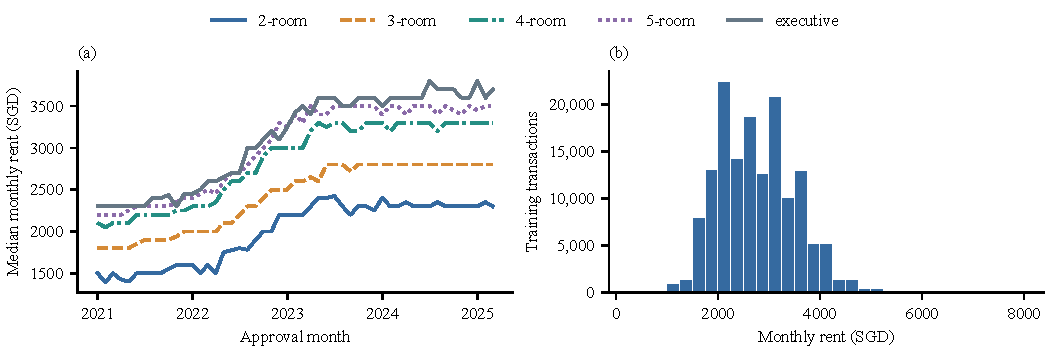
\includegraphics[width=\textwidth]{figures/data_profile.pdf}
\caption{Training-data profile. Left: monthly median rent by canonical flat type; one-room flats are omitted because there are only 42 training observations. Right: the distribution of all 150,000 training rents. Temporal curves describe changing transaction samples, not repeat-flat or causal price indices.}
\label{fig:profile}
\end{figure*}

\subsection{Cleaning guided by exploratory analysis}
We lowercase categories, trim whitespace, replace punctuation with spaces and collapse repeated spaces. For example, \code{3-room} and \code{3 room} become the same category. Raw flat-type labels reduce from eleven to six and street labels from 1,146 to 576 in training. Identical deterministic rules apply to training and competition inputs. This prevents formatting variants from fragmenting comparable groups while preserving immutable raw CSVs.

Furnishing status and fee are constant and are dropped. Calendar year, month, quarter, a month index and nonnegative lease age are derived. Lease age uses the recorded lease commencement year; it is not renovation condition or tenancy duration. Address combines normalised block and street. Block joins also use town and enforce many-to-one matching, preventing accidental row multiplication.

CatBoost receives canonical strings explicitly identified as categorical columns. Linear and Ridge baselines use training-fitted one-hot encoding with unknown values ignored, median imputation and numeric scaling. The scikit-learn tree baselines use training-fitted ordinal encoding, an unknown-category sentinel and numeric median imputation. XGBoost uses native categorical splits with vocabularies fitted on training only. These representations and model capacities differ, so the baseline comparison does not isolate algorithm choice alone.

Fig.~\ref{fig:profile} motivates two subsequent choices. Monthly medians change markedly, making time-invariant group averages inadequate as the only predictor. Flat-type differences also persist, motivating market normalisation within flat type rather than pooling all room counts into one index. Neither descriptive pattern identifies a causal effect, because transaction composition changes over time.

\subsection{Repeated inputs and extreme rents}
An initial audit finds 425 exactly repeated labelled rows. Equal recorded fields and rent are not sufficient evidence of the same flat or contract, so these observations remain. Normalised feature vectors can also repeat with substantially different rents. Removing such records would change the frequency of transaction types without resolving absent individual-flat identity.

Low rents for larger flats motivate a sensitivity study. A fixed rule flags three-room-or-larger or executive observations below half the median for the same approval month, town and canonical flat type. It flags 954 training rows, or 0.636\%. Such a target-defined flag is a diagnostic or training-policy intervention; it cannot be computed from an unlabelled test transaction. We evaluate alternative training policies on the same complete local validation population and preserve every competition row in its original order. We neither label all low rents as errors nor multiply them by a presumed room count.

\section{Methods}
\subsection{Spatial information and baseline learners}
Block features include coordinates, maximum floor, completion year, subzone, planning area and region. Great-circle distances connect each block to the nearest MRT station, mall and primary school; counts within 0.5, 1 and 2 km describe nearby amenities. These are geographic proxies rather than walking or transit travel times. Predictive association with proximity must not be described as a causal premium.

Global and town/flat-type medians establish simple references. Linear Regression, Ridge, Decision Tree, Random Forest and histogram gradient boosting span increasingly flexible approaches. Random Forest\cite{Breiman_2001} supplies a nonlinear bagged-tree reference. CatBoost\cite{NEURIPS2018_14491b75} handles the mixture of numeric and high-cardinality categorical variables and becomes our selected learner after empirical comparison. Later, XGBoost\cite{Chen_2016} receives the same constructed inputs to test learner complementarity. These choices do not imply that CatBoost is universally best.

\subsection{Past-only comparable statistics}
For query month $t$, historical features use only permitted training transactions strictly earlier than $t$. No query-month rent, including a training row's own rent, enters its statistics. For group $g$, an initial smoothed mean is
\begin{equation}
\widehat\mu_{g,t}=\frac{\sum_{i\in H_{g,t}}y_i+\lambda\mu_t}{|H_{g,t}|+\lambda},\quad\lambda=20,
\end{equation}
where $H_{g,t}$ is the earlier group history and $\mu_t$ the earlier global mean. Log support counts accompany these means. Groups include town/type, address/type, address/type/rounded area, street/type and town/type/model, as well as broader groups. These keys identify comparables, not unique flats. Empty early history remains missing with explicit support information; adaptive levels use a fixed 2,000 SGD cold-start prior.

Unadjusted historical rents confound local premium with market movement. Our adaptive representation divides each reference rent by its own flat-type/month mean. It estimates decayed premiums and shrinks specific groups toward parents: town/type, town/street/type, address/type, and address/type/area. Weights $w_i=2^{(m_i-a)/12}$ are anchored at the latest permitted reference month $a$, giving
\begin{equation}
\widehat r_{g,t}=\frac{\sum_{i\in H_{g,t}}w_i r_i+\alpha_g\widehat r_{p(g),t}}{\sum_{i\in H_{g,t}}w_i+\alpha_g}.
\label{eq:premium}
\end{equation}
Here $r_i$ is the reference rent ratio, the top-level parent premium is one, and the four shrinkage strengths are 30, 12, 8 and 5. Anchoring weights to the latest observation avoids making effective support vanish merely because the query is distant. Each group supplies its market-adjusted level, premium, effective support and observation age.

For each flat type, the market forecast begins with the count-weighted mean of the latest three observed monthly means. A log-linear slope uses up to twelve months, requires at least six, and is clipped to $[-0.01,0.01]$ per month. For horizon $h$ from the final reference month,
\begin{equation}
\widehat M_{f,t}=M_{f,a}\exp\!\left[\beta_f\,6(1-e^{-h/6})\right].
\end{equation}
Multiplying this forecast by \eqref{eq:premium} gives a comparable-market level. Damping limits extrapolation but does not eliminate regime risk. These coefficients are recorded design choices rather than parameters fitted to outer validation labels.

\subsection{Local trends and training-history diversity}
Four town/flat-type features capture movement relative to the flat-type market: normalised premium in the latest six reference months, premium in the preceding six, their log ratio clipped to $[-0.15,0.15]$, and log support based on the smaller period count. Both period ratios shrink toward one with strength 20. Thus the method measures local relative momentum rather than fitting an unconstrained future trend independently for each block.

A second training view simulates stale information. Eligible observations are copied with the latest six months of reference labels hidden, while preserving their actual query dates. Eligibility requires at least twelve months since the first reference month. The original and copy each receive half the observation's original weight, preserving total weight. This creates alternative information conditions, not new independent rental evidence. At inference, all components use the full permitted training history for each query.

Each view has a direct rent model $f$ and a model $g$ for residual $y-b_v(x)$, where $b_v(x)$ is the adaptive address/type/area level. Averaging both target modes over seeds 42 and 2026 yields
\begin{equation}
\begin{aligned}
\widehat y(x)&=\frac{1}{8}\sum_v\sum_s
\left[f_{v,s}(x)+b_v(x)+g_{v,s}(x)\right],\\
v&\in\{\mathrm{normal},\mathrm{stale}\},\quad s\in\{42,2026\}.
\end{aligned}
\end{equation}
The normal view includes local trends; the augmented view uses hierarchical features without those four trend columns. Component input dimensions are 78 and 74 respectively. Equal weights preserve diversity without fitting another layer to the latest evaluation errors. Fig.~\ref{fig:pipeline} makes the component count explicit; ``head'' below denotes a view/target pair averaged over its two seeds.

\begin{figure}[t]
\centering
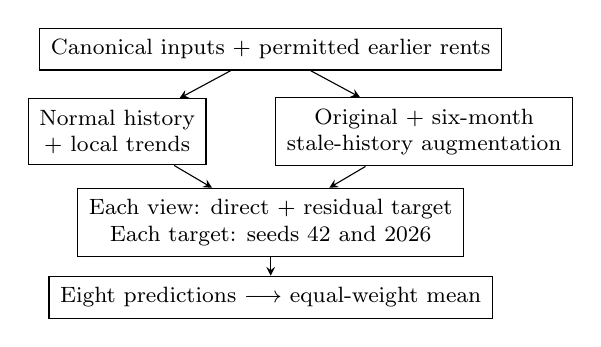
\begin{tikzpicture}[every node/.style={draw,align=center,font=\footnotesize,inner sep=4pt},>=stealth]
\node (input) at (0,0) {Canonical inputs + permitted earlier rents};
\node (normal) at (-1.95,-1.05) {Normal history\\+ local trends};
\node (stale) at (1.95,-1.05) {Original + six-month\\stale-history augmentation};
\node (models) at (0,-2.2) {Each view: direct + residual target\\Each target: seeds 42 and 2026};
\node (output) at (0,-3.15) {Eight predictions $\longrightarrow$ equal-weight mean};
\draw[->] (input) -- (normal); \draw[->] (input) -- (stale);
\draw[->] (normal) -- (models); \draw[->] (stale) -- (models);
\draw[->] (models) -- (output);
\end{tikzpicture}
\caption{Selected model. Augmentation preserves each original transaction's total weight. At inference, both views use the full permitted history.}
\label{fig:pipeline}
\end{figure}

\subsection{Alternative hypotheses}
Stacking\cite{Wolpert_1992} uses predictions generated by earlier training origins to fit a second layer. We compare four seed-averaged heads with all eight individual outputs, using constrained weighting or Ridge correction. Meta-training always precedes meta-evaluation. The retained probe fits nonnegative sum-to-one four-head weights on October--December 2024 and shrinks them halfway toward equal weights; January--March 2025 labels are not used to fit those weights.

Further bounded screens test nearest comparables, flat-type specialists, probabilistically routed rent-band experts, five-fold cross-fitted statistics, honest out-of-fold (OOF) residual corrections and matched-input learners. OOF predictions come from models not fitted on the predicted row's label. Corrections learn earlier-origin OOF residuals rather than fitted-training residuals. Validation routing uses observed features and predicted probabilities, never actual query rent. An isolated area/age composition-trend ablation preserves the original history levels and residual offset; an earlier joint change is not treated as an isolated test.

Economic screens use lagged supplied COE and stock summaries, then official CPI and URA private non-landed rental indices. CPI measures consumer prices, while URA measures private housing rather than HDB rents. Release-lagged levels and changes are supplied with missingness and staleness indicators. A separate MRT calendar reconstructs operational stations by rental month and deduplicates interchange names. Opening exposure describes distance-decayed new-line access, recent openings and months since opening. These features test predictive association, not a causal opening effect.

\section{Experimental Design}
\subsection{Local validation and metrics}
Chronological validation reflects the predominantly later competition period without assuming a pure time series. Each local origin fits on earlier months and retains the complete scoring population. The recent quarter uses 141,076 training and 8,924 validation rows. Table~\ref{tab:temporal} adds annual and sixteen-month windows. These windows overlap and have been repeatedly inspected during development; they are not independent replications or untouched final tests.

RMSE emphasises large deviations, MAE measures typical absolute error, and signed bias distinguishes systematic overprediction from underprediction. Error is prediction minus observation. For subgroup $g$, squared-error share is $\sum_{i\in g}(\widehat y_i-y_i)^2/\sum_i(\widehat y_i-y_i)^2$. Counts accompany subgroup scores: high RMSE in a rare group can contribute less total error than moderate RMSE in a common group.

Historical exploration used scoring-window early stopping for CatBoost, with patience 100. Those results are descriptive references, not unbiased final comparisons. Subsequent temporal comparisons fix 1,600 trees per component and supply no outer scoring labels for early stopping. We keep the protocols separate: a changed tree-selection procedure must not be presented as a gain caused solely by a new feature. Neither procedure uses hidden competition labels.

\subsection{Budgets, promotion and uncertainty}
Selected CatBoost settings are learning rate 0.04, depth 8 and leaf $L_2$ regularisation 6. Early recorded alternatives include 1,200 and 1,600 trees at learning rate 0.04, and 2,200 at 0.03 with regularisation 8. We subsequently freeze 1,600 trees so deployment and local comparison use the same fitting budget. Depth-6 models, recent-sample weighting and market-normalised residual targets are bounded checks rather than an exhaustive parameter search.

Tree budgets and the listed alternatives are recorded development comparisons. History shrinkage strengths, the twelve-month half-life and bounded trend damping are pragmatic smoothing choices, held fixed in subsequent comparisons; they were not exhaustively optimised or independently validated. Their formulas permit reproduction without implying optimality. Four- and eight-component ensembles have equal per-component budgets but different total compute, so the ensemble comparison does not isolate diversity from model count.

Later research usually starts with seed 42 on the recent quarter and sixteen-month window. Candidates replace the matching direct/residual pair in the frozen eight-component mainline, or enter a predefined 25\% blend. These are deployment screens, not full eight-component retrainings or equal-compute learner comparisons. A meaningful recent reduction, approximately 2 RMSE, plus a positive long-window gain is required before another seed and further confirmation periods. This gate discourages promoting changes comparable to fitting noise.

Selected paired comparisons resample normalised block-address clusters 1,000 times and recompute RMSE gains, reporting the 2.5th and 97.5th percentiles. These exploratory intervals preserve within-address association but do not remove dependence across months or adjust for multiple candidate searches. They are not uncertainty intervals for future rents or private competition scores. CatBoost GPU reductions can vary across nominally identical fits; saved predictions and source/input hashes support auditability, not bit-identical refitting.

\section{Results and Interpretation}
\begin{table}[t]
\caption{Research decisions and their supporting evidence.}
\label{tab:decisions}\centering\footnotesize
\begin{tabular}{@{}p{.29\columnwidth}p{.64\columnwidth}@{}}
\toprule Observation/question & Response and decision \\\midrule
Fragmented categories & Canonicalise labels and validate spatial joins; retain ambiguous equal rows. \\
Changing rent levels & Normalise comparables within flat type; retain the adaptive reference. \\
Stale prediction history & Augment training and average targets; retain recent gains with older-period caveat. \\
Concentrated errors & Diagnose observable groups; specialist/correction screens fail the joint advancement gate. \\
Complementary predictions? & Test forward stacking and other learners; keep stacking as a small-gain alternative. \\
Unused context & Screen economic indices and dated rail access; no reliable replacement emerges. \\\bottomrule
\end{tabular}
\end{table}
Table~\ref{tab:decisions} links observations to research decisions. The adaptive reference averages direct and residual models over two seeds (four components); history diversity adds augmented-history counterparts (eight). The selected local-trend model changes only the normal-history half by adding four trend features. Stacking changes their combination weights, not the underlying fitted components.

\subsection{Baseline and spatial information}
\begin{table}[t]
\caption{Exploratory core-input references, January--March 2025 (SGD).}
\label{tab:baselines}\centering\small\begin{tabular}{lrr}
\toprule
Historical core model & RMSE & MAE \\
\midrule
Global median & 844.60 & 691.33 \\
Town/type median & 546.81 & 425.11 \\
Linear regression & 523.20 & 373.09 \\
Ridge & 520.01 & 366.58 \\
Decision tree & 485.90 & 358.59 \\
Random forest & 470.19 & 348.52 \\
Histogram boosting & 463.36 & 336.75 \\
CatBoost (core) & 455.71 & 337.09 \\
\bottomrule
\end{tabular}

\par\smallskip\raggedright\footnotesize CatBoost uses scoring-window early stopping; representations and fitting budgets differ across learners. This is exploratory evidence.
\end{table}
In Table~\ref{tab:baselines}, the global median poorly accommodates heterogeneous flats and the changed market. Town/type medians improve markedly, and nonlinear trees improve further under the chosen representations and budgets. Historical spatial ablations give CatBoost core RMSE 455.71, block 454.19, block plus MRT 452.89, block plus malls 453.97, block plus schools 453.71, and all spatial features 452.62. Modest incremental gains do not establish small real-world amenity effects: address categories already encode correlated location information, and snapshots are imperfect proxies.

The detailed-comparable two-seed model reaches 448.06 under historical early stopping. Later fixed-budget adaptive direct/residual averaging gives 445.52 on the same recent rows. These are milestones under different protocols, so their difference is not an isolated feature gain. Table~\ref{tab:temporal} supplies the controlled fixed-budget evidence for subsequent selection.

\begin{table*}[t]
\caption{Fixed-budget development RMSE (SGD); overlapping windows.}
\label{tab:temporal}\centering\small\begin{tabular}{lrrrr}
\toprule
Validation interval & $n$ & Adaptive (4) & Diversity (8) & Local trend (8) \\
\midrule
Jan-Mar 2025 & 8924 & 445.52 & 440.89 & 440.76 \\
Apr 2024-Mar 2025 & 35158 & 469.54 & 466.89 & 466.76 \\
Apr 2023-Mar 2024 & 35882 & 580.54 & 591.08 & 590.35 \\
Dec 2023-Mar 2025 & 47171 & 486.64 & 483.83 & 483.43 \\
\bottomrule
\end{tabular}

\par\smallskip\raggedright\footnotesize Four or eight components, each with 1,600 trees and seeds 42/2026. Outer scoring labels are not used for early stopping. Total compute differs with component count.
\end{table*}

\subsection{Recent gains and an older-period regression}
History diversity reduces adaptive-reference RMSE by 4.63 on the recent quarter, 2.65 on the recent year and 2.81 on sixteen months, but worsens the older year by 10.55. Adding local trends improves diversity by another 0.13, 0.13, 0.74 and 0.40 respectively. The selected recipe therefore still loses 9.81 versus the adaptive reference on the older year. Its older bias is +82.72 SGD, compared with +8.89 for the adaptive reference. Improvement is conditional on market period.

\begin{figure}[t]
\centering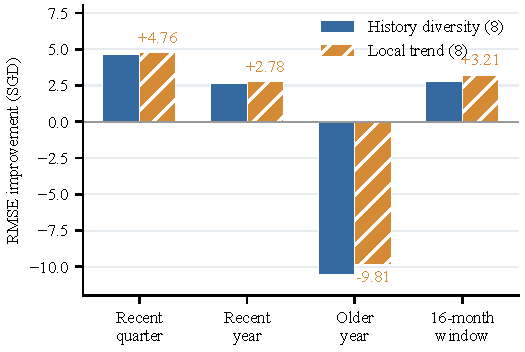
\includegraphics[width=\columnwidth]{figures/temporal_tradeoff.pdf}
\caption{RMSE improvement relative to the four-component adaptive reference. Positive bars mean lower error; both eight-component designs regress on the older year. Categories are separate, overlapping development windows.}
\label{fig:tradeoff}
\end{figure}

The selected recent-quarter RMSE is 440.76, MAE 316.55 and bias +0.79 SGD. Near-zero aggregate bias does not imply calibration within each location or price band. Fig.~\ref{fig:tradeoff} motivates retaining the simpler reference and explicitly acknowledging unresolved temporal sensitivity. Simulating stale history changes the training distribution and can help one regime while overcompensating in another.

We retain the selected model because the later-dated task motivates emphasis on recent conditions, and it improves recent and long-horizon development windows. This is a task-dependent trade-off, not cross-period dominance. In the older year, MAE falls slightly from 455.20 to 454.38 while RMSE rises. This disagreement motivates investigating large residuals rather than assuming every prediction deteriorates; it does not identify their cause. The adaptive reference remains available as a robustness alternative.

\subsection{Stacking and supplementary competition evidence}
Four-head recent-window stacking improves local recent RMSE from 440.7629 to 440.6565, but its paired gain interval $[-0.0342,0.2262]$ crosses zero. The eight-output version instead scores 440.8165. Earlier transfer tests are inconsistent; a sixteen-month stress check loses 0.538 with four inputs and 1.189 with eight. That check changes regime, fitting interval and horizon together, so it does not isolate recency weighting. Stacking remains an alternative rather than the default.

The competition provides an additional observation: team-reported historical public RMSE is 432.14881 for the selected model and 432.04286 for stacking. Test inputs are available, but their rent labels and public-subset membership are hidden. These scores cannot diagnose error mechanisms or replace local evaluation. The public reduction of 0.10595 is consistent with a small gain, yet does not override inconsistent temporal transfer. Full submission history remains in the repository ledger.

An earlier keep-versus-remove sensitivity probe changes public RMSE by only 0.17 in a different model family. It supplies no convincing reason to declare flagged labels wrong. The selected model retains all labels; every local comparison retains its complete scoring population.

\subsection{Where errors concentrate}
\begin{table}[t]
\caption{Recent errors by actual rent (SGD); diagnostic groups only.}
\label{tab:bands}\centering\small\begin{tabular}{lrrrr}
\toprule
Actual rent & $n$ & RMSE & Bias & SSE (\%) \\
\midrule
$\leq$2500 & 1458 & 788.1 & +589.6 & 52.2 \\
2501-3000 & 2525 & 294.4 & +47.3 & 12.6 \\
3001-3500 & 2823 & 276.2 & -113.2 & 12.4 \\
3501-4000 & 1541 & 366.7 & -252.8 & 12.0 \\
$>$4000 & 577 & 568.9 & -456.0 & 10.8 \\
\bottomrule
\end{tabular}

\end{table}
Table~\ref{tab:bands} and Fig.~\ref{fig:errors} show that 1,458 rents at or below 2,500 SGD are 16.34\% of recent rows but contribute 52.23\% of squared error; the corresponding long-window share is 50.86\%. Bias is prediction minus observation. This broad band includes plausible low-priced flats and is not an anomaly label. Low observed rents are overpredicted and high rents generally underpredicted. Conditioning on the realised target itself can contribute to this pattern; the plot alone cannot establish omitted contract conditions or incorrect labels as its cause.

\begin{figure}[t]
\centering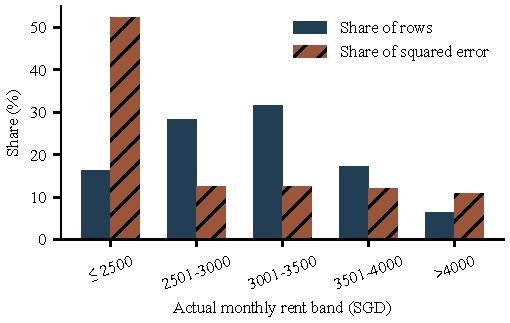
\includegraphics[width=\columnwidth]{figures/error_concentration.pdf}
\caption{Share of recent observations versus share of mainline squared error. The lowest actual-rent band dominates squared error disproportionately. Membership uses observed targets and is unavailable at prediction time.}
\label{fig:errors}
\end{figure}

\begin{table}[t]
\caption{Recent errors by observable flat type (SGD).}
\label{tab:flats}\centering\footnotesize\begin{tabular}{lrrrr}
\toprule
Observed flat type & $n$ & RMSE & Bias & SSE (\%) \\
\midrule
1-room & 4 & 202.5 & -27.8 & 0.0 \\
2-room & 242 & 408.9 & +18.2 & 2.3 \\
3-room & 2,915 & 420.7 & +11.9 & 29.8 \\
4-room & 3,201 & 436.1 & 0.0 & 35.1 \\
5-room & 2,100 & 462.8 & -12.3 & 25.9 \\
executive & 462 & 506.7 & -13.0 & 6.8 \\
\bottomrule
\end{tabular}

\par\smallskip\raggedright\footnotesize All 8,924 validation rows; bias is prediction minus observation. Groups are known at prediction time. The four one-room observations are descriptive only; small contributions may round to zero.
\end{table}
Table~\ref{tab:flats} complements outcome-defined bands. Executive flats have recent RMSE 506.73 across 462 rows, yet only 6.84\% of squared error. Three- and four-room groups together contribute 64.87\%, partly reflecting prevalence. A narrower diagnostic event, actual rent below 65\% of the frozen prediction, occurs in 2.992\% of recent rows and contributes 32.47\% of squared error. A feature-based detector has AUC 0.5761 and average precision 0.04161, versus prevalence 0.02992. This weak ranking signal supports neither reliable hard routing nor a claim that these events are completely unpredictable. Both prevalence and error magnitude matter when selecting a specialist population.

Large errors are therefore not restricted to rare executive flats. Contract terms, condition, renovation, household relationships or label problems are possible explanations for low rents, but none is established by released fields. A target-defined error group helps investigation; it is not itself an operational detector. The next useful analysis should seek a stable observable signal across periods before fitting another specialist.

\subsection{Bounded extensions and negative evidence}\label{sec:extensions}
\begin{table}[t]
\caption{Bounded research screens: RMSE (SGD).}
\label{tab:research}\centering\footnotesize\begin{tabular}{lrr}
\toprule
Candidate applied to mainline & Recent & 16-month \\
\midrule
Nearest-comparable blend & 441.842 & 482.198 \\
Flat-type specialist blend & 441.261 & 483.356 \\
Rent-band mixture blend & 441.962 & 482.488 \\
Cross-fitted statistics & 442.344 & 483.672 \\
Strict-past distribution & 440.641 & 483.299 \\
COE indicators & 440.877 & 483.434 \\
Stock indicators & 440.816 & 483.536 \\
Matched-input XGBoost & 441.881 & 485.244 \\
OOF residual correction & 440.922 & 483.340 \\
Guarded Ridge blend & 442.398 & 481.515 \\
CPI & 440.860 & 483.557 \\
URA rental index & 440.878 & 483.528 \\
Corrected static MRT & 440.631 & 483.418 \\
MRT opening exposure & 440.760 & 483.352 \\
Monthly-available CPI+URA & 440.791 & 483.478 \\
\bottomrule
\end{tabular}

\par\smallskip\raggedright\footnotesize B: 25\% candidate blend; R: replacement of two selected components; C: 25\% OOF residual correction. Screens use one seed and differing budgets.
\end{table}
Table~\ref{tab:research} compares distinct hypotheses, not equal-budget algorithms. Nearest-comparable, specialist and soft-mixture blends can improve sixteen months while losing recently. Matched-input XGBoost worsens both windows; highly correlated prediction errors limit the tested blend's complementarity. This supports retaining the present recipe within the tested budget, not rejecting either algorithm or specialist modelling in general.

Cross-fitting tests a cross-sectional encoding without unique-flat assumptions. Training statistics exclude a held-out inner fold; outer validation uses only outer-training labels. Full-interval cross-fitted statistics worsen both windows. Strict-past dispersion replacement gains only about 0.12 and 0.14 RMSE. The encoding changes training/inference support distributions, so these results apply to the tested configuration. An isolated area/age composition-trend ablation also provides essentially no recent gain and worsens the other main windows.

COE and stock features use preceding-month summaries and origin-frozen controls, but a monthly lag is only a coarse release-time proxy and stock membership is a supplied snapshot. Neither gives a material deployment gain. Ridge reveals a different issue: future numeric inputs can exceed training ranges. Joint clipping to training ranges substantially stabilises its predictions, yet its fixed blend still loses recently while gaining over sixteen months. Since several fields change together, this does not identify one causal extrapolation variable.

For official macro indices, month-start queries activate CPI\cite{cpi} two months after its observation month and URA two months after quarter end. Main screens freeze indices at the validation origin. A same-fitted-model control supplies values released by each rental month, testing contemporaneous covariates rather than a single-origin forecast. Historical revisions and CPI rebasing are not reconstructed: this is latest-vintage, release-lagged evaluation, not fully point-in-time vintages. URA private non-landed rents\cite{ura} are only a proxy for HDB conditions. The monthly CPI+URA replacement remains slightly worse than the mainline on both windows despite improving its own long-window frozen-input control.

The MRT audit finds 55 supplied rows marked open outside the verified operational calendar. The selected model still uses the supplied snapshot, an explicit availability limitation. Research variants verify TEL2--4, Punggol Coast and Hume dates against LTA releases (for example, TEL4\cite{lta}), exclude future/unverified codes, deduplicate interchange names, and activate service from the first full month after opening. Origin-based validation admits dated openings announced before that origin; the monthly-access control admits operational service by the rental month. Supplied coordinates limit coverage, especially for LRT. Corrected static rail gains just 0.1322 and 0.0169 RMSE, with intervals crossing zero. Filtering and deduplication change jointly, so their contributions are not isolated. Dynamic access and opening exposure establish neither a reliable improvement nor a causal premium.

The index and rail studies comprise 36 formal GPU fits, excluding smoke checks. Repeating an otherwise identical seed-42 macro fit changes a replacement score by about 0.13 despite identical input matrices. Improvements at this scale require caution. Correcting station availability improves the meaning of a feature even when it barely changes RMSE; score alone cannot validate historical availability. The selected snapshot remains an offline geographic proxy, not an operational calendar for a live service.

We stop these screens because observed gains are small, unstable across windows or comparable to refit variation. No candidate passes the later advancement gate. The low-rent detector lacks a strong observable signal, and further weight tuning would reuse the same development labels without resolving the older-period failure. This bounded stopping decision preserves evidence for future hypotheses rather than claiming that all useful methods have been exhausted.

\section{Limitations and Reproducibility}
\subsection{Scope of the conclusions}
\textit{Evaluation reuse.} Temporal windows have been inspected repeatedly, several overlap, and public submissions add another selection channel. Bootstrap intervals do not repair this reuse. We have no private-label evaluation. The older-period regression prevents a claim of general dominance over the adaptive reference.

\textit{Incomplete observation.} Unit floor, renovation and contract terms remain unobserved. Ambiguous flat identity and unusual rents establish neither label error nor a population irreducible-error floor. Predictions estimate recorded transactions, not a normative fair rent.

\textit{Information availability.} Static MRT proxies, revised macro vintages, snapshot stock membership and approval/negotiation timing limit live deployment. Spatial and opening associations are not causal estimates.

\textit{Bounded search.} Parameters and representations are not exhaustively explored. One-seed, two-component screens cannot rule out better full retraining. No uncertainty interval for an individual tenancy is supplied. Future work should first identify stable observable subgroup bias in additional, preferably non-overlapping periods, then confirm a promising correction on later data and repeated seeds. Walking access, network connections or commuting time offer transit hypotheses more specific than repeated threshold tuning. These are proposals, not completed experiments.

\subsection{Implementation and reproducibility}
The repository provides reusable code, the selected configuration, cumulative research decisions and score/provenance ledgers. Immutable course data, fitted models and detailed predictions remain local. Authorised readers can regenerate caches using the README; Appendix~\ref{app:reproduce} maps the evidence.

One full-data eight-component fit took 669.44 seconds on an RTX 4060; this is not total research compute. The environment pins Python 3.12 and CatBoost 1.2.10. The recorded implementation passes 55 tests of cutoffs, categories, joins and output protection. Paper assets regenerate from saved evidence without training.

\section{Conclusion}
For RQ1, canonical categories and validated joins establish coherent comparable groups; spatial ablations show modest incremental gains under the tested representation. For RQ2, market-adjusted comparables and history augmentation produce a selected recent RMSE of 440.76 and MAE of 316.55, with additional compute relative to the four-component reference. For RQ3, improvements transfer to two longer development windows but leave an older annual RMSE deficit of 9.81 unresolved. Low observed rents contribute disproportionately to squared error, while current feature-based detection is weak. The resulting lesson is a qualified modeling choice: retain useful recent-market information, document adverse transfer, and seek new observable evidence before further fine tuning.

\clearpage
\IEEEtriggeratref{6}
\bibliographystyle{IEEEtran}
\bibliography{references}
\clearpage
\appendices
\section{Reproduction and Evidence Map}\label{app:reproduce}
Obtain the original course files under \code{data/raw/}, then run \code{python src/check\_setup.py} and \code{python -m pytest -q}. The README supplies full commands to regenerate temporal component predictions before feedback studies. Cached predictions and models are intentionally not distributed with the report. Compiling the committed paper needs only its source and saved aggregate assets; rebuilding experimental evidence additionally needs course data and prediction caches. GPU refits can differ numerically. Frozen hashes and metric checks deliberately reject silently changed evidence; a new run requires a reviewed source manifest and corresponding report update. A clean-machine end-to-end retraining has not been established by this report revision.

Fixed-budget comparisons use \path{src/run_experiments.py} with the \code{--compare-candidates} option. The selected ensemble is generated by \path{src/train_final_model.py} with the recorded configuration; research uses \path{src/feedback_experiments.py}, including \code{--families public} for indices and rail. These are abbreviated entry points; use the complete README commands for exact windows and options.\par
For clarity, the historical core-baseline settings are listed in Table~\ref{tab:parameters}. They are bounded references, not the outcome of an exhaustive or common-compute search. The selected ensemble's settings and history coefficients are given in the main text.
\begin{table}[!ht]
\caption{Principal historical baseline settings; preprocessing is described in the main text.}
\label{tab:parameters}\centering\footnotesize
\begin{tabular}{@{}lp{.61\columnwidth}@{}}
\toprule Model & Recorded settings \\\midrule
Linear/Ridge & Ordinary least squares; Ridge $\alpha=10$ \\
Decision Tree & Maximum depth 18; minimum leaf size 20 \\
Random Forest & 180 trees; maximum feature fraction 0.7; minimum leaf size 3 \\
Histogram boosting & 250 iterations; learning rate 0.08; 31 leaves; $L_2=2$ \\\bottomrule
\end{tabular}
\end{table}
\begin{table}[!ht]
\caption{Evidence locations; detailed local predictions can be regenerated.}
\centering\footnotesize
\begin{tabular}{@{}p{.29\columnwidth}p{.62\columnwidth}@{}}
\toprule Evidence & Location \\\midrule
Baseline/spatial results & \path{reports/experiment_results.csv} \\
Fixed-budget windows & \path{reports/temporal_summary.csv} \\
Research screens & \path{reports/feedback_results.csv} \\
Stacking transfer & \path{reports/stacking_results.csv} \\
Actual public scores & \path{reports/kaggle_submissions.csv} \\
Selected recipe & \path{configs/model.json} \\
Model provenance & \path{reports/final_model_metadata.json} \\
Decisions/limitations & \path{docs/PROGRESS.md} \\\bottomrule
\end{tabular}
\end{table}
\newpage
\section{Team Workload Statement -- To Be Completed}\label{app:workload}
\textit{Reserved for completion before final submission. Responsibilities and contribution proportions have not been assigned in this draft.}
\begin{table}[h]
\caption{Workload placeholder; no contributions are asserted.}
\centering\footnotesize
\begin{tabular}{lll}
\toprule Member & Student ID & Responsibilities \\\midrule
Han Linxuan & A0350911M & To be completed \\
Sun Shenghe & A0354849L & To be completed \\
Zhang Yuhong & A0356795H & To be completed \\
Zhang Zhexuan & A0355290A & To be completed \\\bottomrule
\end{tabular}
\end{table}

\section{AI Assistance}
AI tools assisted with discussion of experimental ideas, code development and checks, interpretation of recorded results, and drafting and editing this report. Numerical results derive from executed experiments and saved evidence; proposed analyses are identified separately. This statement documents assistance under the course policy\cite{policy}; it does not assert that team review or workload attribution has been completed.
\end{document}
